\documentclass[english,a4paper,12pt]{article}
\usepackage[utf8]{inputenc} %for å bruke æøå
\usepackage{babel}
\usepackage{verbatim} %for å inkludere filer med tegn LaTeX ikke liker
\usepackage[document]{ragged2e}
\bibliographystyle{plain}
\usepackage{amsmath}
\usepackage{ulem}
\usepackage[pdftex]{graphicx}
\usepackage{gensymb}
\usepackage{float}
\usepackage{hyperref}
\usepackage{amssymb}
\usepackage[top=0.6in, bottom=0.8in, left=0.9in, right=0.7in]{geometry}
\usepackage{listings}
\usepackage{color}
\usepackage{tikz}

\begin{filecontents}{mybib.bib}
@book{Langtangen-2016,
   author    = "A. Jensen, J. K. Sveen, J. Grue, J.-B. Richon, C. Gray",
   title     = "Accelerations in water waves by extended particle image velocimetry",
   publisher = "Springer-Verlag",
   address   = "\url{}",
   year      = "2001"
}

@unpublished{HLPIV,
   title     = "Getting started with {H}ydrolab{PIV} v1.1",
   author = "Jostein Kolaas, Department of Mathematics, University of Oslo",
   note   = "\url{}"
}

\end{filecontents}
\usepackage{filecontents}
\usepackage{natbib}
\usepackage{bibentry}
\nobibliography*

\title{PIV Project}
\author{Shako Farhad in collaboration with Valentyna Pysarieva \& Farnaz Rezvany}
\date{\today}

\begin{document}

\definecolor{codegreen}{rgb}{0,0.6,0}
\definecolor{codegray}{rgb}{0.5,0.5,0.5}
\definecolor{codepurple}{rgb}{0.58,0,0.82}
\definecolor{backcolour}{rgb}{0.95,0.95,0.92}
 
\lstdefinestyle{mystyle}{
    backgroundcolor=\color{backcolour},   
    commentstyle=\color{codegreen},
    keywordstyle=\color{magenta},
    numberstyle=\tiny\color{codegray},
    stringstyle=\color{codepurple},
    basicstyle=\footnotesize,
    breakatwhitespace=false,         
    breaklines=true,                 
    captionpos=b,                    
    keepspaces=true,                 
    numbers=left,                    
    numbersep=5pt,                  
    showspaces=false,                
    showstringspaces=false,
    showtabs=false,                  
    tabsize=2
}
 
\lstset{style=mystyle}

\maketitle

\begin{abstract}
We used the HydroLabPIV software to cross-correlate two images of particles in a fluid in a wave-tank. We wanted to compare the horizontal velocity profile to the theoretical horizontal velocity profile so that we could see what sub-window size was the most optimal. To be able to compare the numerical horizontal velocity profile to the theoretical one, we had to find the horizontal profile at the crest of the wave. This was done by using the fact that the vertical velocity is approximately zero at the crest. The results show that the experimental data fits very well with the theoretical model when we choose a sub-window size of 46x46 in pixels.
\end{abstract}

\section*{Introduction}
There are many ways to measure fluid motion, one of which is particle image velocimetry (PIV). This is a
non-intrusive optical measurement method, which gives velocity fields resolved in both time and space. \\ \bigskip

To visualize the flow, natural or added tracer particles are usually suspended in the fluid. While the use of particles is the most common, it is also possible to use dye patterns. If the particles are small and/or neutrally buoyant the particles are deemed passive and will follow the fluid motion. The light source we have used is a thin sheath of white LED light. Using light sheet optics the beams are spread to illuminated the field of view, which is captured by a high speed digital camera synchronized with the laser, resulting in a sequence of frames {\cite{HLPIV}}. \\ \bigskip

The software used has been developed at the University of Oslo and is named HLPIV, or HydrLabPIV. We are using this to cross-correlate two images taken with a high-speed camera. This cross-correlation is then used to compare the horizontal speed of the fluid at the crest to theoretical models.

\section*{Theoretical models and methods}
First we created a mask for each image to make the software ignore the boundary at the top. These masks were created in paint by simply marking the area and filling it with black. After reading the four images into the matlab program, we also read the coordinate image to the program. With this coordinate image, we created the physical coordinate system.

\begin{figure}[H]
    \centering
    \includegraphics[width=120mm]{Particles_Masks.png}
    \caption{The black and white image next to the wave with particles is the corresponding mask of that image. The images show water in wave motion with particles in it.}
    \label{fig:1}
\end{figure}

\begin{figure}[H]
    \centering
    \includegraphics[width=120mm]{mpwoco.png}
    \caption{Points have been drawn on the tank, each 5 cm apart. From the surface to the first points it is also 5 cm.}
    \label{fig:2}
\end{figure}

We decided to find the highest horizontal velocity by using the fact that the vertical velocity is zero at the crest. We found where this crest is located by looking for where the vertical velocity is the smallest. This was all found by using cross-correlation and our sub-window had an overlap of 50\%. Then we compared the horizontal velocity to the theoretical model given below.


\begin{equation} \label{eq:wave}
a\cdot \omega\cdot e^{k\cdot z}, \quad \text{where} \quad a = 0.0205m, \quad \omega = 8.95s^{-1}, \quad k = 7.95m^{-1}
\end{equation}

Here $a$ is the amplitude, $\omega$ is the wave frequency, $k$ is the wave-number and $z$ is the vertical coordinates. The physical quantities of these values were given beforehand. 

\section*{Results}
Below we have the results from comparing the numerical horizontal velocity with the theoretical horizontal velocity. In each plot the sub-window size has been reduced and the search range is always one-third of the sub-window size. This is done to find the optimal sub-window size and search range, such that we get as accurate as possible.

\begin{figure}[H]
    \centering
    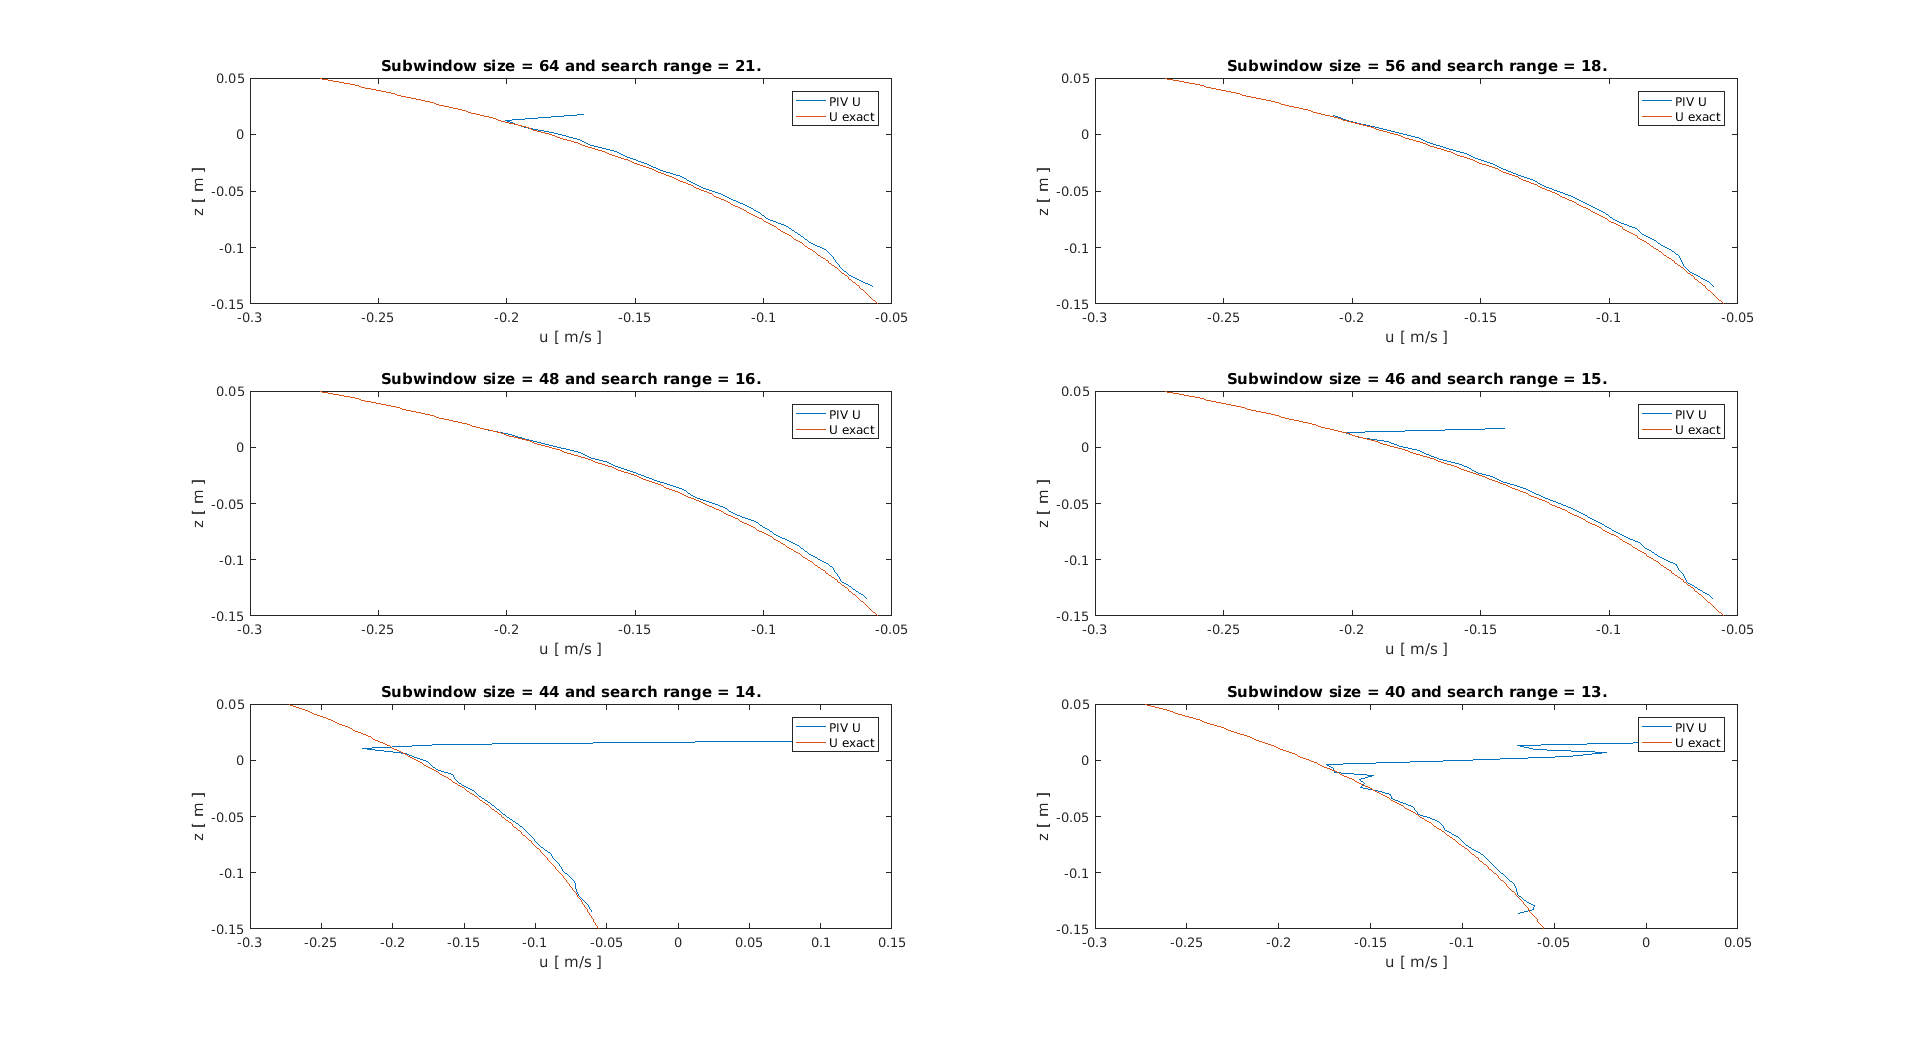
\includegraphics[width=180mm]{PIV_U_vs_U_exact.png}
    \caption{Every graph shows the horizontal velocity profile given from the cross-correlation and from the exact theoretical model. The coordinate-system is in physical coordinates. After we get close to a sub-window size of 46 pixels, we start to see instabilities. These instabilities become more pronounced the smaller we make the sub-window size.}
    \label{fig:3}
\end{figure}

\section*{Discussion}
While the HydroLabPIV software was not always easy to use, we did manage to get some results from it. We could have varied the search ranges and had another figure to look at where instabilities were created. Maybe even tried to vary the overlap percentage, which we had set to 50\% throughout. \\\bigskip

Another problem we had was to compare the theoretical model with the numerical results to find some kind of error. In figure \ref{fig:3} both the second and third plots with sub-window size 56 and 48 respectively, are very similar. If we could compare the theoretical model with the numerical results better, we could have made a better choice of sub-window size.

\section*{Conclusion}
We were restricted by low resolution images, and the minimum quantity of images to do these experiments. But nevertheless the experimental data from the wave-tank behaves very well according to the theoretical model. From the results the best size of the sub-window is 46x46 in pixels. The results also show that we can use the theoretical models to make predictions about the physical world. The difference in the theoretical model and numerical results can be equated to an array of errors that occurs when measuring (taking pictures) and calculating (truncation error etc).

\section*{Appendix}
For matlab code, images and tex source code, see the link below:

\url{https://github.com/ShakoFarhad/PIV-Project-1}

\bibliographystyle{plainnat}
\bibliography{mybib} \bigskip \bigskip
\end{document}
